% Options for packages loaded elsewhere
\PassOptionsToPackage{unicode}{hyperref}
\PassOptionsToPackage{hyphens}{url}
%
\documentclass[
  ignorenonframetext,
]{beamer}
\usepackage{pgfpages}
\setbeamertemplate{caption}[numbered]
\setbeamertemplate{caption label separator}{: }
\setbeamercolor{caption name}{fg=normal text.fg}
\beamertemplatenavigationsymbolsempty
% Prevent slide breaks in the middle of a paragraph
\widowpenalties 1 10000
\raggedbottom
\setbeamertemplate{part page}{
  \centering
  \begin{beamercolorbox}[sep=16pt,center]{part title}
    \usebeamerfont{part title}\insertpart\par
  \end{beamercolorbox}
}
\setbeamertemplate{section page}{
  \centering
  \begin{beamercolorbox}[sep=12pt,center]{part title}
    \usebeamerfont{section title}\insertsection\par
  \end{beamercolorbox}
}
\setbeamertemplate{subsection page}{
  \centering
  \begin{beamercolorbox}[sep=8pt,center]{part title}
    \usebeamerfont{subsection title}\insertsubsection\par
  \end{beamercolorbox}
}
\AtBeginPart{
  \frame{\partpage}
}
\AtBeginSection{
  \ifbibliography
  \else
    \frame{\sectionpage}
  \fi
}
\AtBeginSubsection{
  \frame{\subsectionpage}
}
\usepackage{amsmath,amssymb}
\usepackage{lmodern}
\usepackage{iftex}
\ifPDFTeX
  \usepackage[T1]{fontenc}
  \usepackage[utf8]{inputenc}
  \usepackage{textcomp} % provide euro and other symbols
\else % if luatex or xetex
  \usepackage{unicode-math}
  \defaultfontfeatures{Scale=MatchLowercase}
  \defaultfontfeatures[\rmfamily]{Ligatures=TeX,Scale=1}
\fi
\usetheme[]{Copenhagen}
\usecolortheme{dolphin}
\usefonttheme{structurebold}
% Use upquote if available, for straight quotes in verbatim environments
\IfFileExists{upquote.sty}{\usepackage{upquote}}{}
\IfFileExists{microtype.sty}{% use microtype if available
  \usepackage[]{microtype}
  \UseMicrotypeSet[protrusion]{basicmath} % disable protrusion for tt fonts
}{}
\makeatletter
\@ifundefined{KOMAClassName}{% if non-KOMA class
  \IfFileExists{parskip.sty}{%
    \usepackage{parskip}
  }{% else
    \setlength{\parindent}{0pt}
    \setlength{\parskip}{6pt plus 2pt minus 1pt}}
}{% if KOMA class
  \KOMAoptions{parskip=half}}
\makeatother
\usepackage{xcolor}
\newif\ifbibliography
\usepackage{color}
\usepackage{fancyvrb}
\newcommand{\VerbBar}{|}
\newcommand{\VERB}{\Verb[commandchars=\\\{\}]}
\DefineVerbatimEnvironment{Highlighting}{Verbatim}{commandchars=\\\{\}}
% Add ',fontsize=\small' for more characters per line
\usepackage{framed}
\definecolor{shadecolor}{RGB}{248,248,248}
\newenvironment{Shaded}{\begin{snugshade}}{\end{snugshade}}
\newcommand{\AlertTok}[1]{\textcolor[rgb]{0.94,0.16,0.16}{#1}}
\newcommand{\AnnotationTok}[1]{\textcolor[rgb]{0.56,0.35,0.01}{\textbf{\textit{#1}}}}
\newcommand{\AttributeTok}[1]{\textcolor[rgb]{0.77,0.63,0.00}{#1}}
\newcommand{\BaseNTok}[1]{\textcolor[rgb]{0.00,0.00,0.81}{#1}}
\newcommand{\BuiltInTok}[1]{#1}
\newcommand{\CharTok}[1]{\textcolor[rgb]{0.31,0.60,0.02}{#1}}
\newcommand{\CommentTok}[1]{\textcolor[rgb]{0.56,0.35,0.01}{\textit{#1}}}
\newcommand{\CommentVarTok}[1]{\textcolor[rgb]{0.56,0.35,0.01}{\textbf{\textit{#1}}}}
\newcommand{\ConstantTok}[1]{\textcolor[rgb]{0.00,0.00,0.00}{#1}}
\newcommand{\ControlFlowTok}[1]{\textcolor[rgb]{0.13,0.29,0.53}{\textbf{#1}}}
\newcommand{\DataTypeTok}[1]{\textcolor[rgb]{0.13,0.29,0.53}{#1}}
\newcommand{\DecValTok}[1]{\textcolor[rgb]{0.00,0.00,0.81}{#1}}
\newcommand{\DocumentationTok}[1]{\textcolor[rgb]{0.56,0.35,0.01}{\textbf{\textit{#1}}}}
\newcommand{\ErrorTok}[1]{\textcolor[rgb]{0.64,0.00,0.00}{\textbf{#1}}}
\newcommand{\ExtensionTok}[1]{#1}
\newcommand{\FloatTok}[1]{\textcolor[rgb]{0.00,0.00,0.81}{#1}}
\newcommand{\FunctionTok}[1]{\textcolor[rgb]{0.00,0.00,0.00}{#1}}
\newcommand{\ImportTok}[1]{#1}
\newcommand{\InformationTok}[1]{\textcolor[rgb]{0.56,0.35,0.01}{\textbf{\textit{#1}}}}
\newcommand{\KeywordTok}[1]{\textcolor[rgb]{0.13,0.29,0.53}{\textbf{#1}}}
\newcommand{\NormalTok}[1]{#1}
\newcommand{\OperatorTok}[1]{\textcolor[rgb]{0.81,0.36,0.00}{\textbf{#1}}}
\newcommand{\OtherTok}[1]{\textcolor[rgb]{0.56,0.35,0.01}{#1}}
\newcommand{\PreprocessorTok}[1]{\textcolor[rgb]{0.56,0.35,0.01}{\textit{#1}}}
\newcommand{\RegionMarkerTok}[1]{#1}
\newcommand{\SpecialCharTok}[1]{\textcolor[rgb]{0.00,0.00,0.00}{#1}}
\newcommand{\SpecialStringTok}[1]{\textcolor[rgb]{0.31,0.60,0.02}{#1}}
\newcommand{\StringTok}[1]{\textcolor[rgb]{0.31,0.60,0.02}{#1}}
\newcommand{\VariableTok}[1]{\textcolor[rgb]{0.00,0.00,0.00}{#1}}
\newcommand{\VerbatimStringTok}[1]{\textcolor[rgb]{0.31,0.60,0.02}{#1}}
\newcommand{\WarningTok}[1]{\textcolor[rgb]{0.56,0.35,0.01}{\textbf{\textit{#1}}}}
\setlength{\emergencystretch}{3em} % prevent overfull lines
\providecommand{\tightlist}{%
  \setlength{\itemsep}{0pt}\setlength{\parskip}{0pt}}
\setcounter{secnumdepth}{-\maxdimen} % remove section numbering
\ifLuaTeX
  \usepackage{selnolig}  % disable illegal ligatures
\fi
\IfFileExists{bookmark.sty}{\usepackage{bookmark}}{\usepackage{hyperref}}
\IfFileExists{xurl.sty}{\usepackage{xurl}}{} % add URL line breaks if available
\urlstyle{same} % disable monospaced font for URLs
\hypersetup{
  pdftitle={Hypotheses tests with continuous variables},
  pdfauthor={Alex Sanchez, Miriam Mota, Ricardo Gonzalo and Santiago Perez-Hoyos},
  hidelinks,
  pdfcreator={LaTeX via pandoc}}

\title{Hypotheses tests with continuous variables}
\author{Alex Sanchez, Miriam Mota, Ricardo Gonzalo and\\
Santiago Perez-Hoyos}
\date{Versión 2022-11-23}
\institute{Statistics and Bioinformatics Unit. Vall d'Hebron Institut de
Recerca}

\begin{document}
\frame{\titlepage}

\begin{frame}{Outline}
\protect\hypertarget{outline}{}
\begin{enumerate}
\tightlist
\item
  INTRODUCTION
\item
  TYPE OF TESTS
\item
  NORMALITY TESTS
\item
  ONE GROUP COMPARISON
\item
  TWO GROUPS COMPARISON IN INDEPENDENT SAMPLES
\item
  TWO GROUPS COMPARISON IN DEPENDENT SAMPLES
\item
  \emph{K GROUPS COMPARISON IN INDEPENDENT SAMPLES}
\item
  \emph{Multiple comparisons and multiple testing}
\end{enumerate}
\end{frame}

\begin{frame}{Introduction}
\protect\hypertarget{introduction}{}
\begin{itemize}
\tightlist
\item
  Once the concept of hypothesis testing is established,
\item
  Researchers face the problem of \emph{which test should be applied at
  every possible situation}.
\item
  Best solution:

  \begin{itemize}
  \tightlist
  \item
    understand the problem and the questions addressed
  \item
    know available tests for each problem
  \item
    be aware of applicability assumptions of each test and how to check
    them.
  \end{itemize}
\item
  Easier to say than to do.

  \begin{itemize}
  \tightlist
  \item
    Sometimes cheatsheets may be helpful, but be warned against a blind
    use, that is understand and be critic with the steps.
  \end{itemize}
\end{itemize}
\end{frame}

\begin{frame}{Which test is appropriate for which problem}
\protect\hypertarget{which-test-is-appropriate-for-which-problem}{}
\begin{figure}
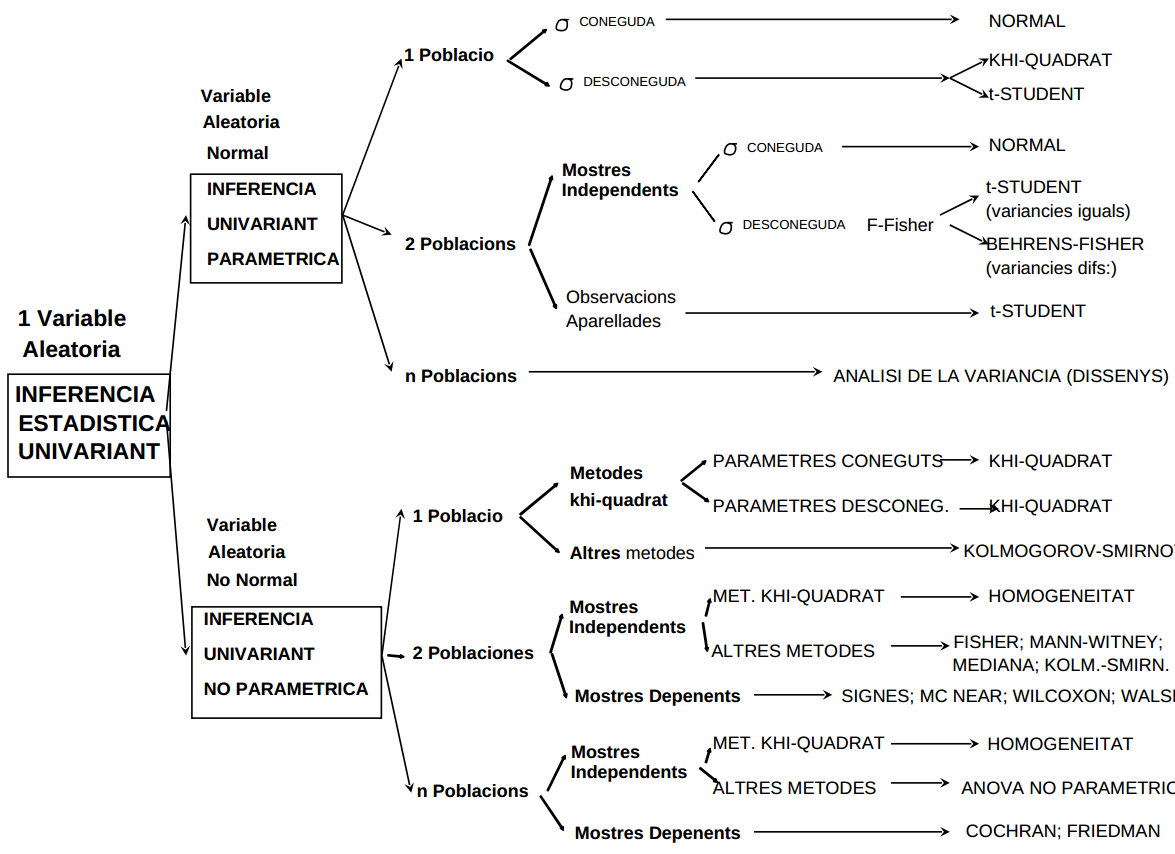
\includegraphics[width=0.8\linewidth]{images/testsXCadaSituacio} \end{figure}
\end{frame}

\begin{frame}{Example situation}
\protect\hypertarget{example-situation}{}
\begin{itemize}
\tightlist
\item
  A study was designed to compare two distinct hypertension control
  programs.
\item
  60 individuals with HTA were randomly assigned to either one or the
  other group (30 per group)
\item
  Blood pressure was measured each month during a year
\end{itemize}
\end{frame}

\begin{frame}[fragile]
\begin{Shaded}
\begin{Highlighting}[]
\NormalTok{hta }\OtherTok{\textless{}{-}} \FunctionTok{read\_excel}\NormalTok{(}\StringTok{"datasets/hta.xls"}\NormalTok{)}
\FunctionTok{print}\NormalTok{(}\FunctionTok{head}\NormalTok{(hta[,}\DecValTok{1}\SpecialCharTok{:}\DecValTok{7}\NormalTok{]))}
\end{Highlighting}
\end{Shaded}

\begin{verbatim}
## # A tibble: 6 x 7
##   numero sexo  grupo  tas1  tad1  tas2  tad2
##    <dbl> <chr> <chr> <dbl> <dbl> <dbl> <dbl>
## 1      1 VARON B       150   100   150    90
## 2      2 MUJER B       160    90   170    90
## 3      3 MUJER B       150    90   110    90
## 4      4 VARON A       120    80   140    90
## 5      5 MUJER A       150    85   145    85
## 6      6 MUJER B       140    75   160    70
\end{verbatim}
\end{frame}

\begin{frame}[fragile]{Always start looking at the data}
\protect\hypertarget{always-start-looking-at-the-data}{}
\tiny

\begin{Shaded}
\begin{Highlighting}[]
\NormalTok{oldpar}\OtherTok{\textless{}{-}}\FunctionTok{par}\NormalTok{(}\AttributeTok{mfrow=}\FunctionTok{c}\NormalTok{(}\DecValTok{1}\NormalTok{,}\DecValTok{1}\NormalTok{)) }\CommentTok{\# Guarda los parámetros para el dibgujo}
\FunctionTok{par}\NormalTok{(}\AttributeTok{mfrow=}\FunctionTok{c}\NormalTok{(}\DecValTok{2}\NormalTok{,}\DecValTok{2}\NormalTok{)) }\CommentTok{\# Dibuja cuatro gráficos por grafico}
\FunctionTok{with}\NormalTok{(hta, }\FunctionTok{boxplot}\NormalTok{(tas1, }\AttributeTok{main=}\StringTok{"Box{-}plot"}\NormalTok{) )}
\FunctionTok{with}\NormalTok{(hta, }\FunctionTok{hist}\NormalTok{(tas1) )}
\FunctionTok{with}\NormalTok{(hta, }\FunctionTok{qqnorm}\NormalTok{(tas1, }\AttributeTok{main=}\StringTok{"Normal QQplot"}\NormalTok{) );}\FunctionTok{with}\NormalTok{(hta, }\FunctionTok{qqline}\NormalTok{(tas1) )}
\FunctionTok{par}\NormalTok{(oldpar) }\CommentTok{\# Vuelve a los parámetros de dibujo originales}
\end{Highlighting}
\end{Shaded}
\end{frame}

\begin{frame}[fragile]{Normality Test}
\protect\hypertarget{normality-test}{}
\small

\begin{Shaded}
\begin{Highlighting}[]
\FunctionTok{with}\NormalTok{(hta,}\FunctionTok{shapiro.test}\NormalTok{(tad1) ) }\CommentTok{\# Shapiro Wilk test}
\end{Highlighting}
\end{Shaded}

\begin{verbatim}
## 
##  Shapiro-Wilk normality test
## 
## data:  tad1
## W = 0.96622, p-value = 0.09512
\end{verbatim}
\end{frame}

\begin{frame}[fragile]{One sample Test}
\protect\hypertarget{one-sample-test}{}
\small

\begin{Shaded}
\begin{Highlighting}[]
\FunctionTok{with}\NormalTok{(hta,}\FunctionTok{t.test}\NormalTok{(tad1,}\AttributeTok{mu=}\DecValTok{90}\NormalTok{) ) }\CommentTok{\# One sample T.test}
\end{Highlighting}
\end{Shaded}

\begin{verbatim}
## 
##  One Sample t-test
## 
## data:  tad1
## t = -1.2137, df = 59, p-value = 0.2297
## alternative hypothesis: true mean is not equal to 90
## 95 percent confidence interval:
##  85.80626 91.02707
## sample estimates:
## mean of x 
##  88.41667
\end{verbatim}
\end{frame}

\begin{frame}[fragile]{Homogeneity variance Test}
\protect\hypertarget{homogeneity-variance-test}{}
\small

\begin{Shaded}
\begin{Highlighting}[]
\FunctionTok{library}\NormalTok{(car)}
\NormalTok{hta}\SpecialCharTok{\%\textgreater{}\%} 
  \FunctionTok{group\_by}\NormalTok{(sexo) }\SpecialCharTok{\%\textgreater{}\%} 
  \FunctionTok{summarise}\NormalTok{(}\AttributeTok{var =} \FunctionTok{sd}\NormalTok{(tas1)) }
\end{Highlighting}
\end{Shaded}

\begin{verbatim}
## # A tibble: 2 x 2
##   sexo    var
##   <chr> <dbl>
## 1 MUJER  17.6
## 2 VARON  22.1
\end{verbatim}

\begin{Shaded}
\begin{Highlighting}[]
\FunctionTok{with}\NormalTok{(hta,}\FunctionTok{leveneTest}\NormalTok{(tad1}\SpecialCharTok{\textasciitilde{}}\FunctionTok{factor}\NormalTok{(sexo),}\AttributeTok{center=}\StringTok{"median"}\NormalTok{))}
\end{Highlighting}
\end{Shaded}

\begin{verbatim}
## Levene's Test for Homogeneity of Variance (center = "median")
##       Df F value Pr(>F)
## group  1  1.3506 0.2499
##       58
\end{verbatim}

\begin{itemize}
\tightlist
\item
  p value is over 0.05
\item
  We can assume homogeneity of variances
\end{itemize}
\end{frame}

\begin{frame}[fragile]{T test when variances are equal}
\protect\hypertarget{t-test-when-variances-are-equal}{}
\small

\begin{Shaded}
\begin{Highlighting}[]
\FunctionTok{with}\NormalTok{(hta,}\FunctionTok{t.test}\NormalTok{(tas1}\SpecialCharTok{\textasciitilde{}}\FunctionTok{factor}\NormalTok{(sexo),}\AttributeTok{var.equal=}\ConstantTok{TRUE}\NormalTok{ ))}
\end{Highlighting}
\end{Shaded}

\begin{verbatim}
## 
##  Two Sample t-test
## 
## data:  tas1 by factor(sexo)
## t = -0.2471, df = 58, p-value = 0.8057
## alternative hypothesis: true difference in means between group MUJER and group VARON is not equal to 0
## 95 percent confidence interval:
##  -11.603461   9.053519
## sample estimates:
## mean in group MUJER mean in group VARON 
##            149.5946            150.8696
\end{verbatim}

\begin{itemize}
\tightlist
\item
  Type I Error is over than 0.05
\item
  We cannot reject mean equality
\end{itemize}
\end{frame}

\begin{frame}[fragile]{T test when variances are unequal}
\protect\hypertarget{t-test-when-variances-are-unequal}{}
\small

\begin{Shaded}
\begin{Highlighting}[]
\FunctionTok{with}\NormalTok{(hta,}\FunctionTok{t.test}\NormalTok{(tas1}\SpecialCharTok{\textasciitilde{}}\FunctionTok{factor}\NormalTok{(sexo),}\AttributeTok{var.equal=}\ConstantTok{FALSE}\NormalTok{ ))}
\end{Highlighting}
\end{Shaded}

\begin{verbatim}
## 
##  Welch Two Sample t-test
## 
## data:  tas1 by factor(sexo)
## t = -0.23436, df = 39.098, p-value = 0.8159
## alternative hypothesis: true difference in means between group MUJER and group VARON is not equal to 0
## 95 percent confidence interval:
##  -12.277927   9.727986
## sample estimates:
## mean in group MUJER mean in group VARON 
##            149.5946            150.8696
\end{verbatim}

\begin{itemize}
\tightlist
\item
  Same conclusions as before
\item
  Test is also known as Welch test
\end{itemize}
\end{frame}

\begin{frame}[fragile]{U Mann-Whitney or Sum Rank non parametric test}
\protect\hypertarget{u-mann-whitney-or-sum-rank-non-parametric-test}{}
\small

\begin{Shaded}
\begin{Highlighting}[]
\FunctionTok{with}\NormalTok{(hta,}\FunctionTok{wilcox.test}\NormalTok{(tad1}\SpecialCharTok{\textasciitilde{}}\FunctionTok{factor}\NormalTok{(sexo)}
\NormalTok{    ,}\AttributeTok{alternative=}\StringTok{\textquotesingle{}two.sided\textquotesingle{}}\NormalTok{,}\AttributeTok{exact=}\ConstantTok{TRUE}\NormalTok{, }\AttributeTok{correct=}\ConstantTok{FALSE}\NormalTok{))}
\end{Highlighting}
\end{Shaded}

\begin{verbatim}
## 
##  Wilcoxon rank sum test
## 
## data:  tad1 by factor(sexo)
## W = 434, p-value = 0.8955
## alternative hypothesis: true location shift is not equal to 0
\end{verbatim}

\begin{Shaded}
\begin{Highlighting}[]
\NormalTok{hta}\SpecialCharTok{\%\textgreater{}\%} 
  \FunctionTok{group\_by}\NormalTok{(sexo) }\SpecialCharTok{\%\textgreater{}\%} 
  \FunctionTok{summarise}\NormalTok{(}\AttributeTok{median =} \FunctionTok{median}\NormalTok{(tad1)) }
\end{Highlighting}
\end{Shaded}

\begin{verbatim}
## # A tibble: 2 x 2
##   sexo  median
##   <chr>  <dbl>
## 1 MUJER     90
## 2 VARON     90
\end{verbatim}

\begin{itemize}
\tightlist
\item
  Null Hypothesis cannot be rejected
\end{itemize}
\end{frame}

\begin{frame}[fragile]{Paired T-test}
\protect\hypertarget{paired-t-test}{}
\small

\begin{Shaded}
\begin{Highlighting}[]
\FunctionTok{with}\NormalTok{(hta,}\FunctionTok{t.test}\NormalTok{(tas1,tas12,}\AttributeTok{paired=}\ConstantTok{TRUE}\NormalTok{))}
\end{Highlighting}
\end{Shaded}

\begin{verbatim}
## 
##  Paired t-test
## 
## data:  tas1 and tas12
## t = 6.0672, df = 51, p-value = 1.609e-07
## alternative hypothesis: true mean difference is not equal to 0
## 95 percent confidence interval:
##   8.518285 16.943253
## sample estimates:
## mean difference 
##        12.73077
\end{verbatim}

\begin{Shaded}
\begin{Highlighting}[]
\FunctionTok{summary}\NormalTok{(hta}\SpecialCharTok{$}\NormalTok{tas1)}
\end{Highlighting}
\end{Shaded}

\begin{verbatim}
##    Min. 1st Qu.  Median    Mean 3rd Qu.    Max. 
##   100.0   140.0   145.0   150.1   160.0   210.0
\end{verbatim}

\begin{Shaded}
\begin{Highlighting}[]
\FunctionTok{summary}\NormalTok{(hta}\SpecialCharTok{$}\NormalTok{tas12)}
\end{Highlighting}
\end{Shaded}

\begin{verbatim}
##    Min. 1st Qu.  Median    Mean 3rd Qu.    Max.    NA's 
##   110.0   130.0   139.0   137.2   150.0   175.0       8
\end{verbatim}

\begin{itemize}
\tightlist
\item
  P value is over 0.05
\end{itemize}
\end{frame}

\begin{frame}[fragile]{Paired Sign-Rank Wilcoxon Test}
\protect\hypertarget{paired-sign-rank-wilcoxon-test}{}
\small

\begin{Shaded}
\begin{Highlighting}[]
\FunctionTok{with}\NormalTok{(hta,}\FunctionTok{wilcox.test}\NormalTok{(tad1,tad12,}
     \AttributeTok{exact=}\ConstantTok{TRUE}\NormalTok{, }\AttributeTok{paired=}\ConstantTok{TRUE}\NormalTok{))}
\end{Highlighting}
\end{Shaded}

\begin{verbatim}
## 
##  Wilcoxon signed rank test with continuity correction
## 
## data:  tad1 and tad12
## V = 478.5, p-value = 0.05333
## alternative hypothesis: true location shift is not equal to 0
\end{verbatim}
\end{frame}

\begin{frame}[fragile]{Read diabetes data}
\protect\hypertarget{read-diabetes-data}{}
\tiny

\begin{Shaded}
\begin{Highlighting}[]
\FunctionTok{library}\NormalTok{(readxl)}
\FunctionTok{library}\NormalTok{(dplyr)}
\FunctionTok{library}\NormalTok{(magrittr)}
\NormalTok{diabetes }\OtherTok{\textless{}{-}} \FunctionTok{read\_excel}\NormalTok{(}\StringTok{"datasets/diabetes.xls"}\NormalTok{)}
\FunctionTok{sapply}\NormalTok{(diabetes, class)}
\end{Highlighting}
\end{Shaded}

\begin{verbatim}
##    numpacie        mort    tempsviu        edat         bmi    edatdiag 
##   "numeric" "character"   "numeric"   "numeric"   "numeric"   "numeric" 
##       tabac         sbp         dbp         ecg         chd 
## "character"   "numeric"   "numeric" "character" "character"
\end{verbatim}

\begin{Shaded}
\begin{Highlighting}[]
\NormalTok{diabetes\_factor }\OtherTok{\textless{}{-}}\NormalTok{ diabetes }\SpecialCharTok{\%\textgreater{}\%}
  \FunctionTok{mutate\_if}\NormalTok{(}\FunctionTok{sapply}\NormalTok{(diabetes, is.character), as.factor) }\SpecialCharTok{\%\textgreater{}\%}
  \FunctionTok{select}\NormalTok{ (}\SpecialCharTok{{-}}\NormalTok{numpacie)}

\NormalTok{diabetes}\SpecialCharTok{\%\textgreater{}\%} 
  \FunctionTok{group\_by}\NormalTok{(ecg) }\SpecialCharTok{\%\textgreater{}\%} 
  \FunctionTok{summarise}\NormalTok{( }\AttributeTok{n=}\FunctionTok{n}\NormalTok{(),}
    \AttributeTok{mean =} \FunctionTok{mean}\NormalTok{(edat),}
            \AttributeTok{sd=}\FunctionTok{sd}\NormalTok{(edat)) }
\end{Highlighting}
\end{Shaded}

\begin{verbatim}
## # A tibble: 3 x 4
##   ecg          n  mean    sd
##   <chr>    <int> <dbl> <dbl>
## 1 Anormal     11  64.9  6.76
## 2 Frontera    27  53.8 11.4 
## 3 Normal     111  50.5 11.5
\end{verbatim}
\end{frame}

\begin{frame}[fragile]{ANOVA}
\protect\hypertarget{anova}{}
\begin{Shaded}
\begin{Highlighting}[]
\NormalTok{anova}\OtherTok{\textless{}{-}}\FunctionTok{aov}\NormalTok{(edat}\SpecialCharTok{\textasciitilde{}}\NormalTok{ecg,}\AttributeTok{data=}\NormalTok{diabetes\_factor)}
\FunctionTok{summary}\NormalTok{(anova)}
\end{Highlighting}
\end{Shaded}

\begin{verbatim}
##              Df Sum Sq Mean Sq F value  Pr(>F)    
## ecg           2   2166  1083.0   8.619 0.00029 ***
## Residuals   146  18347   125.7                    
## ---
## Signif. codes:  0 '***' 0.001 '**' 0.01 '*' 0.05 '.' 0.1 ' ' 1
\end{verbatim}
\end{frame}

\begin{frame}[fragile]{Multicomparison}
\protect\hypertarget{multicomparison}{}
\tiny

\begin{Shaded}
\begin{Highlighting}[]
\FunctionTok{library}\NormalTok{(multcomp)}
\NormalTok{tuk }\OtherTok{\textless{}{-}} \FunctionTok{glht}\NormalTok{(anova, }\AttributeTok{linfct =} \FunctionTok{mcp}\NormalTok{(}\AttributeTok{ecg =} \StringTok{"Tukey"}\NormalTok{))}

  \FunctionTok{print}\NormalTok{(}\FunctionTok{summary}\NormalTok{(tuk)) }\CommentTok{\# pairwise tests}
\end{Highlighting}
\end{Shaded}

\begin{verbatim}
## 
##   Simultaneous Tests for General Linear Hypotheses
## 
## Multiple Comparisons of Means: Tukey Contrasts
## 
## 
## Fit: aov(formula = edat ~ ecg, data = diabetes_factor)
## 
## Linear Hypotheses:
##                         Estimate Std. Error t value Pr(>|t|)    
## Frontera - Anormal == 0  -11.094      4.010  -2.767 0.016509 *  
## Normal - Anormal == 0    -14.405      3.543  -4.065 0.000215 ***
## Normal - Frontera == 0    -3.310      2.405  -1.376 0.345708    
## ---
## Signif. codes:  0 '***' 0.001 '**' 0.01 '*' 0.05 '.' 0.1 ' ' 1
## (Adjusted p values reported -- single-step method)
\end{verbatim}
\end{frame}

\begin{frame}[fragile]
\tiny

\begin{Shaded}
\begin{Highlighting}[]
  \FunctionTok{print}\NormalTok{(}\FunctionTok{confint}\NormalTok{(tuk, }\AttributeTok{level=}\FloatTok{0.95}\NormalTok{)) }\CommentTok{\# confidence intervals}
\end{Highlighting}
\end{Shaded}

\begin{verbatim}
## 
##   Simultaneous Confidence Intervals
## 
## Multiple Comparisons of Means: Tukey Contrasts
## 
## 
## Fit: aov(formula = edat ~ ecg, data = diabetes_factor)
## 
## Quantile = 2.3459
## 95% family-wise confidence level
##  
## 
## Linear Hypotheses:
##                         Estimate lwr      upr     
## Frontera - Anormal == 0 -11.0943 -20.5009  -1.6876
## Normal - Anormal == 0   -14.4046 -22.7173  -6.0919
## Normal - Frontera == 0   -3.3103  -8.9534   2.3328
\end{verbatim}
\end{frame}

\begin{frame}[fragile]{Multicomparison plot}
\protect\hypertarget{multicomparison-plot}{}
\small

\begin{Shaded}
\begin{Highlighting}[]
  \FunctionTok{plot}\NormalTok{(}\FunctionTok{confint}\NormalTok{(tuk))}
\end{Highlighting}
\end{Shaded}
\end{frame}

\begin{frame}[fragile]{Kruskal-Wallis Test}
\protect\hypertarget{kruskal-wallis-test}{}
\small

\begin{Shaded}
\begin{Highlighting}[]
\NormalTok{diabetes\_factor}\SpecialCharTok{\%\textgreater{}\%} 
  \FunctionTok{group\_by}\NormalTok{(ecg) }\SpecialCharTok{\%\textgreater{}\%} 
  \FunctionTok{summarise}\NormalTok{(}\AttributeTok{median =} \FunctionTok{median}\NormalTok{(edat)) }
\end{Highlighting}
\end{Shaded}

\begin{verbatim}
## # A tibble: 3 x 2
##   ecg      median
##   <fct>     <dbl>
## 1 Anormal      64
## 2 Frontera     53
## 3 Normal       49
\end{verbatim}

\begin{Shaded}
\begin{Highlighting}[]
\FunctionTok{kruskal.test}\NormalTok{(edat}\SpecialCharTok{\textasciitilde{}}\NormalTok{ecg,}\AttributeTok{data=}\NormalTok{diabetes\_factor)}
\end{Highlighting}
\end{Shaded}

\begin{verbatim}
## 
##  Kruskal-Wallis rank sum test
## 
## data:  edat by ecg
## Kruskal-Wallis chi-squared = 17.483, df = 2, p-value = 0.0001598
\end{verbatim}
\end{frame}

\begin{frame}[fragile]{Dunn Test for multiple comparison}
\protect\hypertarget{dunn-test-for-multiple-comparison}{}
\small

\begin{Shaded}
\begin{Highlighting}[]
\FunctionTok{library}\NormalTok{(dunn.test)}
\FunctionTok{with}\NormalTok{(diabetes\_factor,}\FunctionTok{dunn.test}\NormalTok{(edat,ecg,}\AttributeTok{method=}\StringTok{"bonferroni"}\NormalTok{))}
\end{Highlighting}
\end{Shaded}

\begin{verbatim}
##   Kruskal-Wallis rank sum test
## 
## data: edat and ecg
## Kruskal-Wallis chi-squared = 17.4826, df = 2, p-value = 0
## 
## 
##                            Comparison of edat by ecg                           
##                                  (Bonferroni)                                  
## Col Mean-|
## Row Mean |    Anormal   Frontera
## ---------+----------------------
## Frontera |   2.721182
##          |    0.0098*
##          |
##   Normal |   4.075469   1.467464
##          |    0.0001*     0.2134
## 
## alpha = 0.05
## Reject Ho if p <= alpha/2
\end{verbatim}
\end{frame}

\end{document}
